\section{LBM Solver and Benchmarking}\label{sec:lbm-benchmark}

In \cref{sec:lbm-intro} we introduced the basic mechanics and governing equations behind mass, momentum, and energy transport with the lattice-Boltzmann method. In summary, there are two main requirements to the definition of a lattice-Boltzmann model: a collision operator, $\Omega_i$, and the constants which define the structural framework of the lattice, $q$, $\vec{c}_i$, $c_s$, and $w_i$.

\begin{figure}[t]
	\centering
	\caption{A representative node with directional vectors to the 8 neighbors (+1 central node) in the D2Q9 lattice.}
	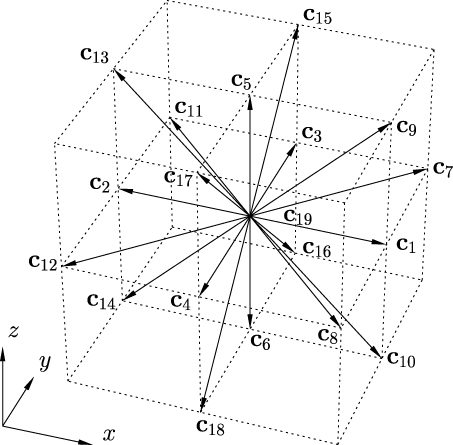
\includegraphics[width=\singleimagewidth]{chapters/figures/lbm/4193301.jpg}\label{fig:d2q9-lattice}
\end{figure}

The computational domain of the fluid is discretized into a Cartesian grid with regularized spacing, $\delta_x$, in every dimension. At each node is a density function, $f_i(\vec{x},t)$, which represent the density at that node (found at $\vec{x}$), traveling in the direction of $\vec{c}_i$ at a moment in time, $t$. We will be solving the equations through a three-dimensional pebble bed, but use a common two-dimensional lattice for demonstration purposes. Given in Fig.~\ref{fig:d2q9-lattice} is a node in a D2Q9 lattice; the directions and lengths of the velocity vectors are shown.

The density distribution function evolves according to Eq.~\ref{eq:lbm-evolution}. It is given again here for reference,
\begin{align}
	\underbrace{f_i(\vec{x}+\vec{c}_i, t + 1)  = f_i(\vec{x},t)}_\text{streaming}  + \underbrace{\Omega_i(\vec{x},t)}_\text{collision}
\end{align}

Conceptually the evolution can be thought of as two distinct operations. First, the collision operator is calculated based only on each nodes local information. Using the BGK approximation, given in Eq.~\ref{eq:bgk-operator}, the collision is calculated as
\begin{align}
	\Omega_i = -\frac{1}{\tau}\left[f_i(\vec{x},t) - f_i^\eq(\vec{x},t)\right]
\end{align}

Post-collision, in the streaming step, the information is passed from the node to its neighbors along the lattice directions shown in Fig.~\ref{fig:d2q9-lattice}. While the collision operation is exactly local, the streaming operation involves only nearest neighbors. After the streaming step, the nodes that lie along the boundary have some particle distributions that are unknown as their neighbors lie outside the domain. In these cases, the bounce-back boundary condition is applied wherein distributions arriving at the boundary are reflected back to their incident directions. The bounce-back calculation enforces no-slip at the walls.

Splitting the evolution of the distribution function into the two steps of collision and streaming, in addition to being a conceptual aid, is a natural partition of computational steps. In practice the algorithm proceeds as follows,\cite{Viggen2009}
\begin{enumerate}
\item{\textbf{Equilibrium}: Using macroscopic properties of density and fluid velocity, the equilibrium distribution function is calculated at every node following Eq.~\ref{eq:equilib-dist-function}}
\item{\textbf{Collision}: The BGK collision operator is calculated according to Eq.~\ref{eq:bgk-operator} to find the post-collision distribution of every node}
\item{\textbf{Streaming}: Information from each node propagates to neighboring nodes based on the evolution equation of Eq.~\ref{eq:lbm-evolution}.}
\item{\textbf{Macroscopic properties}: Updated macroscopic properties are found from the new distribution functions according to Eq.~\ref{eq:lbm2physical}.}
\end{enumerate}

It is worth stressing again that the lattice-Boltzmann calculations are completely local, with the streaming step requiring only inter-node communication for updating distribution functions. 

\subsection{Numerical Solver}

In this work, we make use of the open-source code maintained by FlowKit Ltd named Palabos.\cite{Flow} The Palabos library provides an interface for quick implementation of lattice-Boltzmann models in C++. Implemented models include the BGK and thermal flows with the Boussinesq approximation, among many others. They are all run on the possible grids of D2Q9, D3Q13, D3Q15, D3Q19, or D3Q27. Zou/He, periodic, and bounce-back conditions are built into the LB kernel; implementation of Dirichlet or Neumann conditions with velocity or pressure are possible. The software is freely available under the terms of the open-source AGPLv3 license.\cite{FreeSoftwareFoundationInc.2007} All mentioned models and ingredients are parallelized with MPI, including the I/O operations that are implemented in terms of MPI’s Parallel I/O API.

\subsection{Benchmark Cases}
Before we attempt to implement a coupled flow of the conjugate heat transfer between pebble beds and the interstitial gas, we will solve some simpler benchmark cases.